\chapter{Scaling with reference size} \label{ch:trie}
\graphicspath{{\dir/}}

In this chapter we consider the problem of semi-global alignment of a set of
reads to a general graph reference. We supplement the reference graph with a
trie index and run shortest path algorithms (Dijkstra and \A with a very simple
heuristic) that start aligning from the trie root. We demonstrate that using a
trie index enables sublinear scaling of the alignment time with the reference
size. Even for moderate size references, we rearch orders of magnitude of
speedup compared to other optimal algorithms.

% This text will be sanitized and placed into lqa-output/abstract.txt
%
Motivation and approach: the trie index works for scaling sublinerly with the
reference size but each error in the query triggers deeper exploration of the
trie so the runtime grows exponentially. Lets inform the \A algorithm using
information from the whole query length while keeping the trie. This way we
could avoid the deep trie exploration and scale to long queries (as far as the
error rate is not too high).

We present a novel \A \emph{\seedh} that enables fast and optimal
sequence-to-graph alignment, guaranteed to minimize the edit distance of the
alignment assuming non-negative edit costs.

We phrase optimal alignment as a shortest path problem and solve it by
instantiating the \A~algorithm with our \seedh. The \seedh first extracts
non-overlapping substrings (\emph{seeds}) from the read, finds exact seed
\emph{matches} in the reference, marks preceding reference positions by
\emph{crumbs}, and uses the crumbs to direct the \A search. The key idea is to
punish paths for the absence of foreseeable seed matches. We prove admissibility
of the \seedh, thus guaranteeing alignment optimality.

\qquad Our implementation extends the free and open source aligner and
demonstrates that the \seedh outperforms all state-of-the-art optimal aligners
including \graphaligner, \vargas, \pasgal, and the \prefixh previously employed
by \astarix. Specifically, we achieve a consistent speedup of >60$\times$ on
both short Illumina reads and long HiFi reads (up to 25kbp), on both the
\textit{E.~coli} linear reference genome (1Mbp) and the MHC variant graph
(5Mbp). Our speedup is enabled by the \seedh consistently skipping >99.99\% of
the table cells that optimal aligners based on dynamic programming
compute.\\

\astarix aligner and evaluations: \astarixurl\\

Genome graph, Optimal alignment, Semi-global alignment, Edit distance, Shortest
path, Long reads, \A algorithm, Seed heuristic
\section{Overview}

% General: aligning, edit distance
Alignment of reads to a reference genome is an essential and early step in most
bioinformatics pipelines. While linear references have been used traditionally,
an increasing interest is directed towards graph references capable of
representing biological variation~\citep{garrison_variation_2018}.
%
Specifically, a \emph{sequence-to-graph} alignment is a base-to-base
correspondence between a given read and a walk in the graph. As sequencing
errors and biological variation result in inexact read alignments, edit distance
is the most common metric that alignment algorithms optimize in order to find
the most probable read origin in the reference.

% We note that in contrast to linear references, reference graphs capture
% genomic variation and therefore enable more accurate
% alignments~\citep{garrison_variation_2018}.

\paragraph{Suboptimal alignment}
%
In the last decades, approximate and alignment-free methods satisfied the demand
for faster algorithms which process huge volumes of genetic
data~\citep{kucherov2019evolution}. 
%
\emph{Seed-and-extend} is arguably the most popular paradigm in read
alignment~\citep{altschul_basic_1990,langmead_fast_2012,li_fast_2009}. First,
substrings (called \emph{seeds} or \emph{kmers}) of the read are extracted, then
aligned to the reference, and finally prospective matching locations are
\emph{extended} on both sides to align the full read.

While such a heuristic may produce acceptable alignments in many cases, it
fundamentally does not provide quality guarantees, resulting in suboptimal
alignment accuracy.
%
In contrast, here we demonstrate that seeds can benefit optimal alignment as
well.

\paragraph{Key challenges in optimal alignment}
%
Finding optimal alignments is desirable but expensive in the worst case,
requiring $\Oh(Nm)$ time~\citep{equi2019complexity}, for graph size $N$ and read
length $m$.
%
Unfortunately, most optimal sequence-to-graph aligners rely on dynamic
programming (DP) and always reach this worst-case asymptotic runtime. Such
aligners include \vargas~\citep{darby2020vargas},
\pasgal~\citep{jain_accelerating_2019},
\graphaligner~\citep{rautiainen_bitparallel_2019},
\hga~\citep{feng2021accelerating}, and \vg~\citep{garrison_variation_2018},
which use bit-level optimizations and parallelization to increase their
throughput.

In contrast, we follow the promising direction of using a heuristic to avoid
worst-case runtime on realistic data. To this end, \astarix rephrases the task
of alignment as a shortest-path problem in an \emph{alignment graph} extended by
a \emph{trie index}, and solves it using the \A~algorithm instantiated with a
problem-specific \prefixh. Importantly, its choice of heuristic only affects
performance, not optimality.
%
Unlike DP-based algorithms, this \prefixh allows scaling sublinearly with the
reference size, substantially increasing performance on large genomes. However,
it can only efficiently align reads of limited length.

\paragraph{Contributions}
%
Here we address the key challenge of scaling to long HiFi reads, while
retaining the superior scaling of \astarix in the size of the reference graph.
%
To this end, we instantiate the \A algorithm with a novel \seedh, which
outperforms existing optimal aligners on both short and long HiFi reads.
%
Specifically, the \seedh utilizes information from the whole read to narrowly
direct the \A search by placing \emph{crumbs} on graph nodes which lead up to a
\emph{seed match}, \ie, an exact match of a substring of the read.

Overall, the contributions presented next include:
\begin{enumerate}
    \item A novel \A~\seedh that exploits information from the whole read to
    quickly align it to a general graphs reference.
    \item An optimality proof showing that the \seedh always finds an alignment
    with minimal edit distance.
	\item An implementation of the \seedh as part of the \astarix aligner.
    \item An extensive evaluation of our approach, showing that we align both
    short Illumina reads and long HiFi reads to both linear and graph references
    $\geq 60 \times$ faster than existing optimal aligners.
    \item A demonstration of superior empirical runtime scaling in the reference
    size $N$: $N^{0.46}$ on Illumina reads and $N^{0.11}$ on HiFi reads.
\end{enumerate}

\begin{figure}[t]
    \centering
	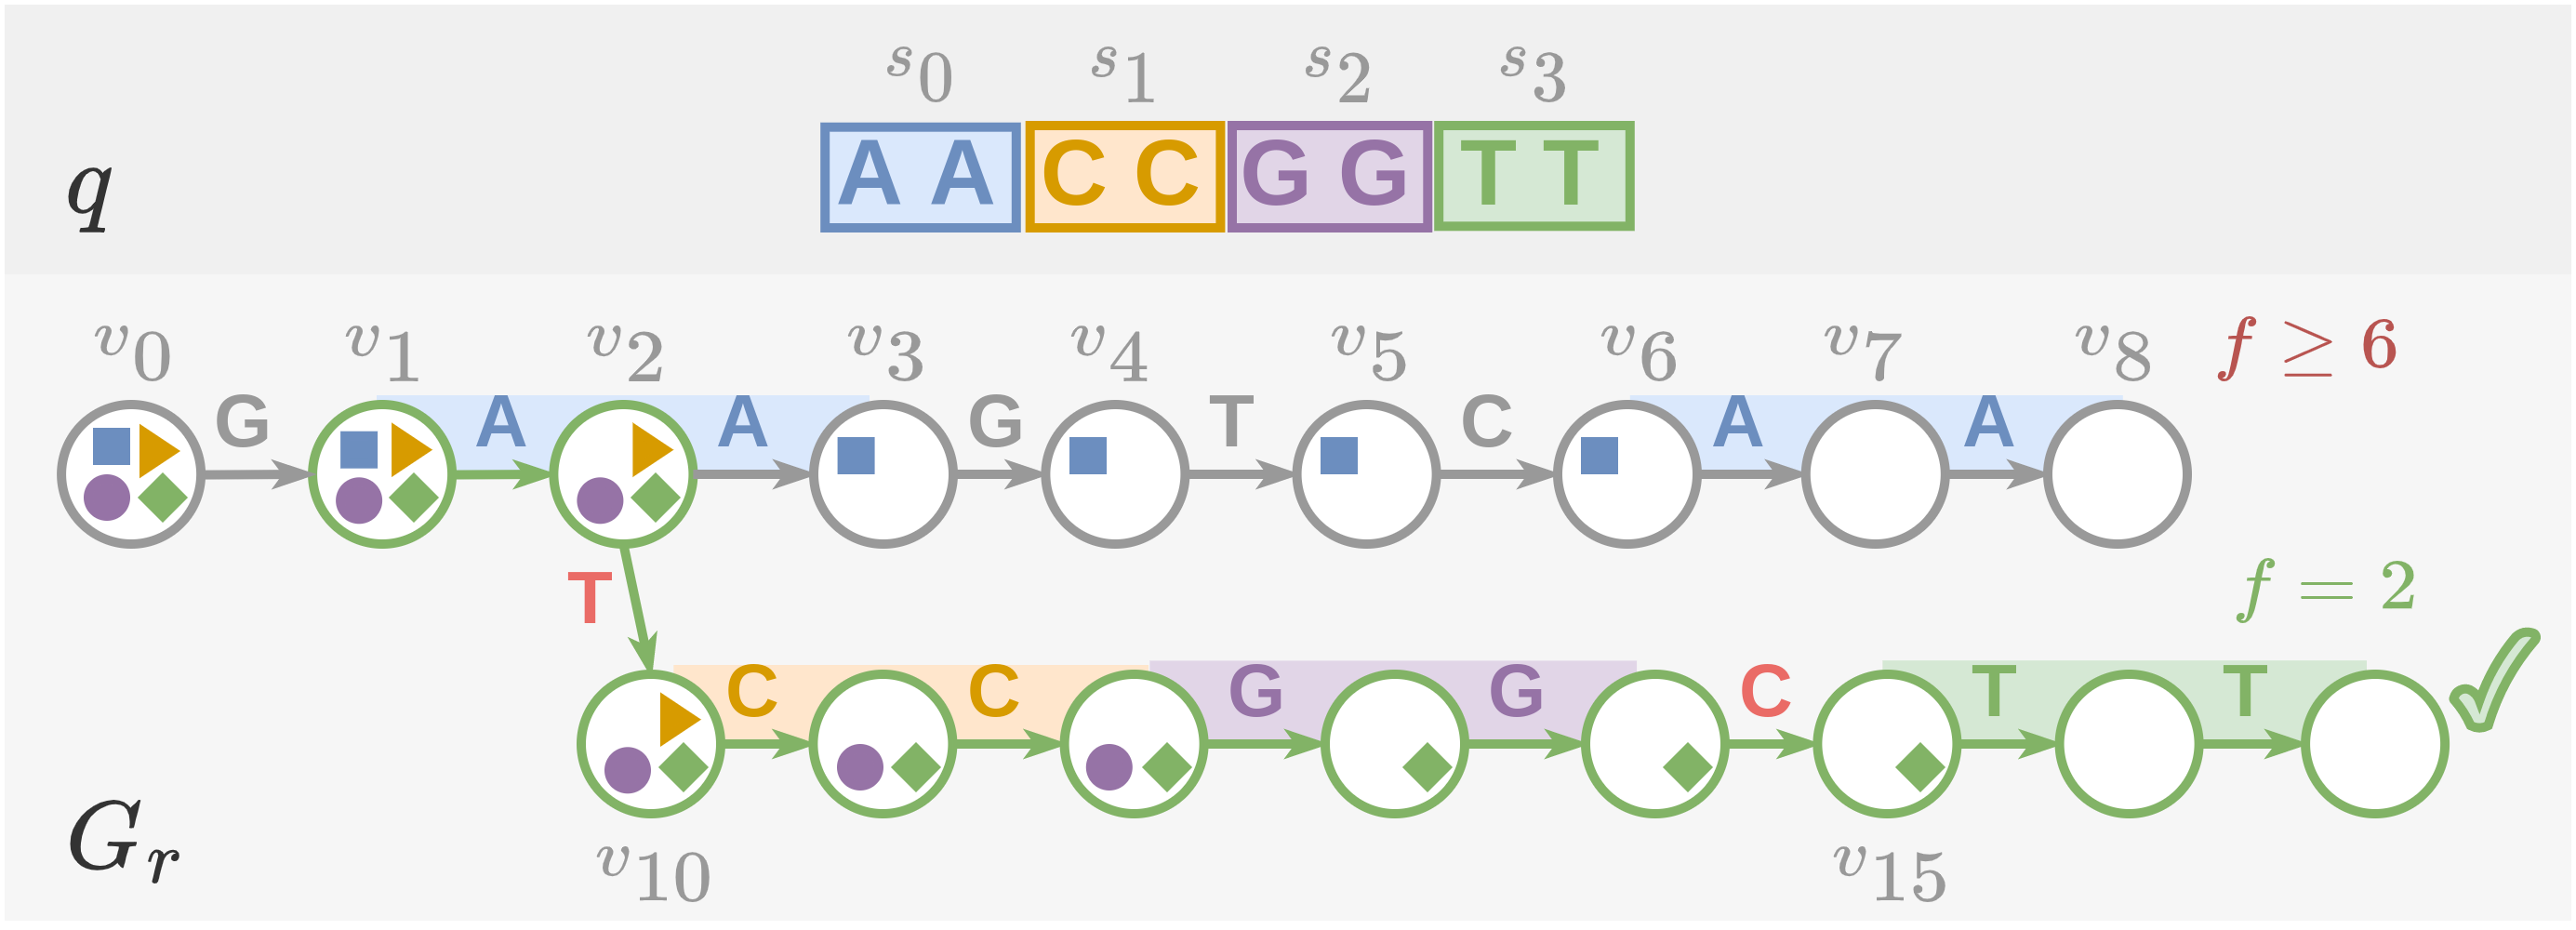
\includegraphics[width=0.6\linewidth]{figures/seed-heuristic-diagram.png}
	\caption{%
		A toy overview example using the \seedh to align a read $q$ to a
		reference graph $\RG$. The read is split into four colored seeds, where
		their corresponding crumbs are shown inside reference graph nodes as
		symbols with matching color. The optimal alignment is highlighted as a
		green path ending with a tick (\protect\greentick{}) and includes one
		substitution
		($\mathtt{\textcolor{dark-red}{T}{\rightarrow}\textcolor{dark-red}{A}}$)
		and one deletion ($\textcolor{dark-red}{\mathtt{C}}$).
		%
	}
\label{SEEDfig:overview}
\end{figure}

\paragraph{Intuition} \label{SEEDsec:overview}
% Task
\cref{SEEDfig:overview} showcases the \sh on an overview example. It shows a
read~$q$ to be aligned to a reference graph~$\RG$. Our goal is to find an
optimal alignment starting from an arbitrary node $v \in \RG$.
%
For simplicity of the exposition, we assume unit edit costs $\cedits =
(0,1,1,1)$, which we generalize in~\cref{SEEDsec:definition}.

\paragraph{Intuition}
The \A search requires us to provide a lower bound of the remaining path cost
from a state $\st{v}{i}$ to a target state. Clearly, to align the whole query,
each of the remaining seeds (\ie~at or after position $i$ in $q$) has to be
eventually aligned. The intuition underlying the \sh is to punish the state
for the absence of any foreseeable match of each remaining seed. Notice that the
order of the seeds is not directly taken into account.

In order to quickly check if a seed $s$ can lead to a match, we follow a
procedure similar to the one used by Hansel and Gretel who were placing
breadcrumbs to find their trail back home. Before aligning a query, we will
precompute all $\emph{crumbs}$ from all seeds so that not finding a crumb for
a seed $s$ on node $v$ indicates that seed $s$ could not be matched exactly
before the query is fully aligned continuing from $v$. This way, assuming that a
shortest path includes many seed matches, the crumbs will direct the \A search
along with it.

If a crumb from an expected seed is missing in node $v$, its corresponding seed
$s$ could not possibly be aligned exactly and this will incur the cost of at
least one substitution, insertion, or deletion. Assuming unit edit costs,
$h\st{v}{i}$ yields a lower bound on the cost for aligning $q[i{:}]$ starting
from $v$ by simply returning the number of missing expected crumbs in $v$.

\paragraph{Crumbs precomputation example}
%
\cref{SEEDfig:overview} shows four seeds as colored sections of length $2$ each, and
represents their corresponding crumbs as \bluecrumb{}, \yellowcrumb{},
\violetcrumb{} and \greencrumb{}, respectively. Four crumbs are expected if we
start at $v_2$, but \bluecrumb{} is missing, so $h\st{v_2}{0}=1$. Analogously,
if we reach $v_2$ after aligning one letter from the read, we expect 3 crumbs
(except \bluecrumb{}), and we find them all in $v_2$, so $h\st{v_2}{1}=0$.
%
To precompute the crumbs for each seed, we first find all positions in $\RG$
from which the seed aligns exactly. \cref{SEEDfig:overview} shows these exact
matches as colored sections of $\RG$. Then, from each match we traverse $\RG$
backwards and add crumbs to nodes that could lead to these matches.
%
For example, because seed \colorbox{light-yellow}{$\mathtt{CC}$} can be matched
starting in node $v_{10}$, crumbs~\yellowcrumb{} are placed on all nodes leading
up to $v_{10}$.
%
Similarly, seed \colorbox{light-blue}{$\mathtt{AA}$} has two exact matches, one
starting in node $v_{0}$ and one starting in node $v_{6}$.
%
However, we only add crumbs \bluecrumb{} to nodes $v_{0}$, $v_{1}$, and
$v_{3}$--$v_{6}$, but not to node $v_{2}$. This is because $v_{2}$ is
(i)~strictly after the beginning of the match of
\colorbox{light-blue}{$\mathtt{AA}$} at $v_1$ and (ii)~too far before the match
of \colorbox{light-blue}{$\mathtt{AA}$} at $v_{6}$.
%
Specifically, any alignment starting from node $v_{2}$ and still matching
\colorbox{light-blue}{$\mathtt{AA}$} at $v_{6}$ would induce an overall cost of
$4$ (it would require deleting the $4$ letters $A$, $G$, $T$, and $C$). Even
without a crumb \bluecrumb{} on $v_{2}$, our heuristic provides a lower bound on
the cost of such an alignment: it never estimates a cost of more than~$4$, the
number of seeds.

% In contrast to \bluecrumb{}, the crumbs \greencrumb{} for the match of seed
% \colorbox{light-green}{$\mathtt{TT}$} are placed on all nodes before $v_{15}$.
% This is because even when starting from $v_0$, we could match
% \colorbox{light-green}{$\mathtt{TT}$} at $v_{15}$ without a cost exceeding the
% cost of $4$ (by deleting $\mathtt{G}$, substituting
% $\mathtt{\textcolor{dark-red}{T}{\rightarrow}\textcolor{dark-red}{A}}$, and
% deleting $\mathtt{\textcolor{dark-red}{C}}$, at an overall cost of $3$).

\stepcounter{footnote}
\footnotetext{\label{SEEDfootnote:tie-braking}Depending on how the \A~algorithm
handles tie-braking, different sets of states could be explored. For simplicity,
we show all states that \emph{could potentially} be explored.}
\begin{figure}[t]
    \centering
	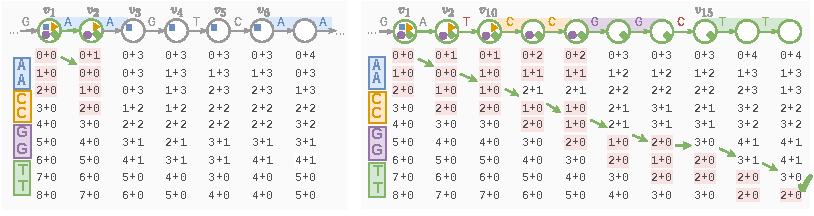
\includegraphics[width=\linewidth]{\dir/figures/seed-heuristic-tables}
	\caption{Exploration of $\AG[q]$, searching for a shortest path from the
	first to the last row using the \seedh. The table entry in the $i^\text{th}$
	row (zero indexed) below node $v$ shows $g\st{v}{i}+h\st{v}{i}$, where
	$g\st{v}{i}$ is the shortest distance from any starting state $\st{u}{0}$ to
	$\st{v}{i}$.
	%
	States that may\textsuperscript{\cref{SEEDfootnote:tie-braking}} be expanded by
	the \A~algorithm are highlighted in \colorbox{pink-highlight}{pink}, and the
	rest of the states are shown for completeness even though they are never
	expanded. The shortest path corresponding to the best alignment is shown
	with green arrows~(\textcolor{dark-green}{$\pmb{\rightarrow}$}).}
	%
	\label{SEEDfig:exploration-table}
\end{figure}


\paragraph{Guiding the search example}
%
\cref{SEEDfig:exploration-table} demonstrates how $h\st{v}{i}$ guides the
\A~algorithm towards the shortest path by showing which states may be
\colorbox{pink-highlight}{expanded} when using the \sh.
%
Specifically, the unique optimal alignment in \cref{SEEDfig:overview} starts from
node $v_{1}$, continues to $v_{2}$, and then proceeds through node $v_{10}$
(instead of~$v_{3}$).

While the \sh initially explores all states of the form $\st{v}{0}$ (we
discuss in \cref{SEEDsec:trie} how to avoid this by using a trie), it skips
expanding any state that involves nodes $v_{3}$--$v_{8}$. This improvement is
possible because all these explored states are penalized by the \sh by at
least $3$, while the shortest path of cost $2$ will be found before considering
states on nodes $v_{3}$--$v_{8}$.
%
Here, the heuristic function accurately predicts that expanding $v_{10}$ may
eventually lead to an exact alignment of seeds
\colorbox{light-yellow}{$\mathtt{CC}$}, \colorbox{light-violet}{$\mathtt{GG}$}
and \colorbox{light-green}{$\mathtt{TT}$}, while expanding $v_3$ may not lead to
an alignment of either seed.
%
In particular, the \sh is not misled by the short-term benefit of correctly
matching $A$ in $v_{2}$, and instead provides a long-term recommendation based
on the whole read. Thus, even though the walk to $v_{3}$ aligns exactly the
first two letters of $q$, \A does not expand $v_{3}$ because the \sh
guarantees that the future cost will be at least $3$.

% Overall, the \sh directs the search to the best alignment with one
% substitution
% ($\mathtt{\textcolor{dark-red}{T}{\rightarrow}\textcolor{dark-red}{A}}$) and
% one deletion ($\textcolor{dark-red}{\mathtt{C}}$).

\section{\astarix: Finding Optimal Alignments Using \A} \label{sec:astarix-algo}
In this section, we first introduce the general \A algorithm for finding
shortest paths, and the notion of an optimistic heuristic, a sufficient
condition for instantiations of \A to be correct (i.e., to indeed find shortest
paths). Then we instantiate \A with our domain-specific heuristic that accounts
for upcoming subsequences to be aligned, and prove that this heuristic is
optimistic.

\begin{algorithm}[t]
	\caption{\astarix including heuristic function.}\label{alg:astarix}
	\begin{algorithmic}[1]
		\State $\RG$: Reference graph \label{lin:reference}
		\Comment Global variables
		\State $d$: Upcoming sequence length \label{lin:d}
		\Statex
		\Function{AStarix}{$q\colon \text{Query}$} \label{lin:astarix}
			\State $\AG \gets \Call{DefineAlignmentGraph}{\RG, q}$
			\Comment Following \cref{sec:task}
			\State $S \gets \{\langle v,i \rangle \in \AGV \mid i=0 \}$ \label{lin:starts}
			\Comment Sources: no letter matched
			\State $T \gets \{\langle v,i \rangle \in \AGV \mid i=|q| \}$
			\Comment Targets: all letters matched
			\State \Return $\Call{\A}{\AG, S, T, \textsc{Heuristic}}$
			\Comment \A provided in \cref{app:astar} \label{lin:ret}
		\EndFunction
		\Statex
		\Function{Heuristic}{$\langle u, i \rangle\colon \text{State}$} \label{lin:heuristic-start}
		\Comment Heuristic: Cost of upcoming sequence
			\State $d' \gets \min(d, |q|-i)$
			\Comment Actual length of upcoming sequence
			\State $s \gets q[i:i+d']$ \label{lin:s}
			\Comment Upcoming sequence (next $d$ letters after current)
			\State \Return $\Call{$h$}{u, s}$
			\label{lin:align-upcoming}
			\Comment Cost of aligning $s$ to $\EG$ starting from $u$
		\EndFunction \label{lin:heuristic-end}
		\Statex
		\Function{$h$}{$u, s$}
		\Comment Cost of aligning $s$ starting from $u$
			\State \Return $\Call{RecursiveAlign}{u, s, 0.0, \infty}$
			\Comment Simple branch-and-bound \label{lin:recursive-align}
		\EndFunction
	\end{algorithmic}
\end{algorithm}
\subsection{Background: General \A algorithm} \label{subsec:general-astar}
Given a weighted graph $G=(V,E)$ with $E \subseteq V \times V \times
\mathbb{R}_{\geq 0}$, the \A algorithm (abbreviated as \A) searches for the
shortest path from sources $S \subseteq V$ to targets $T \subseteq V$. It is an
extension of Dijkstra's algorithm that additionally leverages a \emph{heuristic
function} $h \colon V \to \mathbb{R}_{\geq 0}$ to decide which paths to explore
first.
%
If $h(u) \equiv 0$, \A is equivalent to Dijkstra's algorithm.
%
We provide an implementation of \A and Dijkstra in \cref{app:astar}, but do not
assume knowledge of either algorithm in the following.
%
At a high level, \A maintains the set of all \emph{explored} states, initialized
with the set of sources $S$. Then, \A iteratively \emph{expands} the explored
state with lowest estimated cost by exploring all its neighbors, until it finds
a target. Here, the cost for node $u$ is estimated by the distance from source, called $g(u)$, plus the estimate from the heuristic $h(u)$.


\para{Heuristic Function}
The heuristic function $h(u)$ estimates the
cost $h^*(u)$ of a shortest path in $G$ from $u$ to a target $t \in T$. Intuitively, a
good heuristic correlates well with the distance from $u$ to $t$.

To ensure that \A indeed finds the shortest path, $h$ should be
\emph{optimistic}:

\begin{definition}[Optimistic heuristic] A heuristic $h$ is \textit{optimistic}
    if it provides a lower bound on the distance to the closest target: $\forall u. h(u) \leq h^*(u)$.
\end{definition}

While any optimistic $h$ ensures that \A finds optimal
alignments~\cite{dechter_generalized_1985}, the specific choice of $h$
is critical for performance. In particular, decreasing the error $\delta(u) =
h^*(u)-h(u)$ can only improve the performance of
\A~\cite{dechter_generalized_1985}. Thus, a key contribution of ours is
a domain-specific heuristic $h$.


\subsection{\astarix: Instantiating \A} \label{TRIEsubsec:astarix-heuristic}
\cref{TRIEalg:astarix} shows an unoptimized version of \astarix and its heuristic
function.
%
\astarix expects a reference graph (\cref{TRIElin:reference}) and a query
(\cref{TRIElin:astarix}) as input, and returns an optimal alignment (\cref{TRIElin:ret})
by searching for a shortest path from $S$ to $T$ in the alignment graph $\AG$.
It is parameterized by hyper-parameters ($d$ in \cref{TRIElin:d}, more in
\cref{TRIEsec:optimizations}) and edit costs (implicitly provided).

The function \textsc{Heuristic}
(\crefrange{TRIElin:heuristic-start}{TRIElin:heuristic-end}) computes a lower bound on
the remaining cost of a best alignment: the minimum cost $h(u,s)$ of aligning
the \emph{upcoming sequence} $s$ (where $\lvert s \rvert \leq d$) starting from
node $u$. Importantly, $s$ is limited to the next $d' \leq d$ letters of $q$,
starting from query position $i$. Thus, computing $h(u,s)$ is substantially
cheaper than aligning all remaining letters of $q$.

To compute $h(u,s)$ we leverage a simple branch-and-bound algorithm, provided in
\cref{TRIEapp:recursive-align}. In the following, for convenience, we refer to the
heuristic as $h$ (which is parameterized by $(u,s)$) instead of
\textsc{Heuristic} (which is parameterized by $\langle u, i \rangle$). Further,
we say that $h$ is optimistic if $h(u,s)$ is a lower bound on the cost for
aligning all remaining letters (\ie, $q[i:|q|]$) starting from node $u$ (note
that $s$ is a prefix of $q[i:|q|]$).

\begin{samepage}
\begin{thm} \label{TRIEthm:optimistic}
	$h$ is optimistic.
\end{thm}
\begin{proof}
$h$ only considers the next $d'$ letters of $q$ instead of all
remaining letters. Since all costs are non-negative, the theorem follows.
\end{proof}
\end{samepage}

\begin{figure}[t]
	\centering
	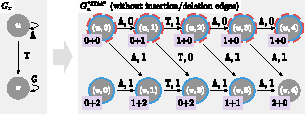
\includegraphics[width=0.9\columnwidth]{figs/heuristic}
	\caption{The benefit of using our heuristic over \dijkstra. Alignment graph
	$\AG[``\texttt{ATAA}"]$ (right) is based on reference graph $\RG$ (left),
	but omits insertion and deletion edges for simplicity. The pink boxes $g+h$
	indicate the distance from the sources $S=\{\langle u,0 \rangle, \langle v,0
	\rangle \}$ (in $g$) and the cost of aligning the next $d=2$ letters (in
	$h$). \dijkstra (resp. \A) expands states circled in
	\textcolor{my-full-blue}{blue} (resp.
	\textcolor{my-full-red}{dashed red}).}
	\label{TRIEfig:heuristic-benefit}
\end{figure}

\para{Benefit of \A Heuristic over \dijkstra} \label{TRIEpara:heuristic-benefits}
\cref{TRIEfig:heuristic-benefit} shows the benefit of using our heuristic function
compared to \dijkstra. Here, \dijkstra expands states based on their distance
$g$ from the origin nodes $\st{u}{0}$ and $\st{v}{0}$. Hence, depending on
tie-breaking, \dijkstra may expand all states with $h \leq 1$, as shown in
\cref{TRIEfig:heuristic-benefit}. By contrast, \A chooses the next state to expand
by the sum of the distance from the origin $g$ and the heuristic $h$, expanding
only states with $g+h \leq 1$.

\para{Memoization} \label{TRIEpara:memoization}
Recall that the return value of $h$ in \cref{TRIElin:heuristic-start} only depends
on $u$ and the upcoming sequence $s$ (which in turn depends on $i$ and $d$).
Thus, $h(u,s)$ can be reused for different positions across different queries in
$\Oh(1)$ time, if it was computed for a previous query.
\section{Optimizations} \label{TRIEsec:optimizations}

We now discuss several optimizations we developed to speed up \astarix while
preserving its optimality. These optimizations reduce preprocessing and
alignment runtime as well as memory footprint (in particular for memoization).
Our aligner \astarix handles both \A and \dijkstra algorithm (formally with $h
\equiv 0$).

\subsection{Greedy match optimization} \label{TRIEsubsec:greedy}
We also employ an optimization originally developed for computing the edit
distance between two strings~\cite{sellers_algorithm_1974,allison_lazy_1992}, but
which has also been used in the context of string to graph
alignment~\cite{dox2018efficient}. We omit the correctness proof of this
optimization, which is already covered
in~\cite{sellers_algorithm_1974}, and only explain the intuition behind it.

Suppose there is only one outgoing edge $e = (u, v, \ell) \in \RGE$ from a node
$u \in \RGV$. Suppose also that while aligning a query $q$, we explore state
$\st{u}{i}$ for which the next query letter $q[i]$ matches the label $\ell$. In
this case, we do not need to consider the edit outgoing edges, because
any edit at this point can be postponed without additional cost, as $\cmatch
\leq \min(\csubst, \cins, \cdel)$. Thus, we can greedily explore state
$\st{v}{i+1}$, aligning $q[i+1]$ to $e$ by using the edge $(\st{u}{i},
\st{v}{i+1}, \ell, \cmatch)$ before continuing with the \A search.
We note that this optimization is only applicable when aligning in non-branching
regions of the reference graph. In particular, it is not applicable for most
trie nodes (\cref{TRIEsubsec:trie}).

\subsection{Capping the cost and depth} \label{TRIEsubsec:speedup-heuristic}
In the following, we show how to reduce the runtime of evaluating the heuristic
$h(u,s)$, by introducing two separate optimizations that compose naturally.

\paragraph{Capping cost} We cap $h(u,s)$ at $\costcap$, replacing it by
$h_{\costcap}(u,s):=\min(h(u,s),\costcap)$. To achieve this, we allow
\textsc{RecursiveAlign} to ignore paths costing more than $\costcap$.
%
For large enough $\costcap$, this speeds up computation without significantly
decreasing the benefit of the heuristic, since nodes associated with a high
heuristic value are typically not explored anyways. We investigate the effect of
$\costcap$ in \cref{TRIEsubsec:parameter_estimation}.

\begin{samepage}
	\begin{thm} \label{TRIEthm:hcostcap_admissible}
		$h_{\costcap}$ is admissible.
	\end{thm}
	\begin{proof}
		Follows from $h_\costcap(u,s) \leq h(u,s)$ and $h(u,s)$ being admissible
		(\cref{TRIEthm:admissible}).
	\end{proof}
	\end{samepage}

\paragraph{Capping depth}
We reduce the number of nodes that need to be considered by $h(u,s)$. To this
end, we define a modified heuristic $h_d(u,s)$ that only considers nodes $R_u
\subseteq \AGV$ at distance at most $d$ from $u$ (in \cref{TRIEalg:astarix}):
$
R_u := \{ v \in \RGV \mid \exists \; \text{path } \pi \in \RG \text{ from } u \text{ to } v \text{ with } \lvert \pi \rvert \leq d \}
$.

If an alignment of $s$ reaches the boundary of $R_u$, defined as $$B(R_u) := \{v
\in R_u \mid \exists (v,v',\ell) \in \AGE \text{ with } v' \notin R_u \},$$ it is
allowed to only spell a prefix of $s$, and the remaining unaligned letters of
$s$ are considered aligned with zero cost:
\begin{gather*}
h_d(u,s) := \min_{\pi \in \Pi} \cost{\pi}, \text{ where } \\
\Pi := \left\{ \pi \in \RG \;\middle|\;
%\begin{array}{c}
\mli{start}(\pi)=u, 
\sigma(\pi)=s \lor \big(\mli{end}(\pi)\in B(R_u) \land \exists i. \sigma(\pi)=s[1..i] \big)
%\end{array}
\right\}
\end{gather*}

\begin{samepage}
\begin{thm} \label{TRIEthm:hbar_admissible}
	$h_d$ is admissible.
\end{thm}
\begin{proof}
	It suffices to show $h_d(u,s) \leq h(u, s)$ since $h(u, s)$ is admissible.
	In the case where all of $s$ is aligned, $h_d(u,s) = h(u, s)$. Otherwise,
	the unaligned letters of $s$ are not penalized, so $h_d(u,s) \leq h(u, s)$.
\end{proof}
\end{samepage}


\subsection{Equivalence classes} \label{TRIEsubsec:partition}

We have shown in \cref{TRIEpara:memoization} how to reuse an already computed
$h(u,s)$ for repeating $s$ across different queries and query positions. In the
following, we additionally aim to reuse $h(u,s)$ across different nodes $u$, so
that $h(u,s)$ does not need to be computed for all nodes $u$. Intuitively, we
want to assign two nodes $u$ and $v$ to the same equivalence class when the
\emph{graph region} considered by $h(u,s)$ is equivalent to the graph region
considered by $h(v,s)$, up to renaming of nodes.

Thus, $h(u,s)=h(v,s)$ if $u$ and $v$ are from the same equivalence class.
Therefore, we can (arbitrarily) choose a representative node $r \in \RGV$ for
every equivalence class, and evaluate $h(r,s)$ instead of $h(u,s)$, where $r$ is
the representative of the equivalence class of $u$. To look up representative
nodes in $\Oh(1)$, we define a helper array $\mli{repr}$ with $\mli{repr[u]} =
r$.

\paragraph{Identifying equivalence classes}
To identify the nodes belonging to the same equivalence class, we assume the
optimization from \cref{TRIEsubsec:speedup-heuristic}, \ie, that our heuristic only
considers nodes up to a distance $d$ from~$u$.
%
Moreover, for performance reasons, our implementation detects only the
equivalence classes of nodes $u$ with a single outgoing path of length at least
$d$.
%
In this case, $u$ and $u'$ are in the same equivalence class if their outgoing
paths spell the same sequence.
%
In contrast, we leave nodes with forking paths in separate equivalence classes.

Note that for smaller $d$, the number of equivalence classes gets smaller, the
reuse of the heuristic gets higher, and the memoization table has a lower memory
footprint. At the same time, however, the heuristic $h_d(u,s)$ is less
informative.

\subsection{Data structures}
Our \astarix implementation uses an adjacency list graph data structure to
represent the reference and the trie in a unified way, representing each letter
by a separate edge object. To represent the reverse complementary walks in
$\RG$, the nodes are doubled, connected in the opposite direction, and
labeled with complementary nucleotides ($\texttt{A} \leftrightarrow \texttt{T}$,
$\texttt{C} \leftrightarrow \texttt{G}$). We do not limit the number of memoized
heuristic function values (\cref{TRIEpara:memoization}), but note we could do so
by resetting the memoization table periodically.
%%%%%%%%%%%%%%%%%%%%%%%%%%%%%%%%%
%\section{Experimental Results}
\section{Evaluation} \label{TRIEsec:eval}
%%%%%%%%%%%%%%%%%%%%%%%%%%%%%%%%%

\begin{samepage}
In this section we present a thorough experimental
evaluation\footnote{\url{https://github.com/eth-sri/astarix/tree/RECOMB2020_experiments}}
of \astarix on simulated Illumina reads. Our evaluation demonstrates that:
\begin{enumerate}
  \item \astarix is faster than \dijkstra because the heuristic reduces the number of explored states by an order of magnitude.
  \item The runtime of \astarix scales better than state-of-the-art optimal
  aligners with increasing graph size, on a variety of reference graphs.
\end{enumerate}
\end{samepage}

\subsection{Implementation \astarix}

Our \astarix implementation uses an adjacency list graph data structure to
represent the reference and the trie in a unified way, representing each letter
by a separate edge object.
%\para{Reverse Complement Alignment}
To represent the reverse complementary walks in $\RG$, the vertices are doubled,
connected in the opposite direction, and labeled with complementary nucleotides
($\texttt{A} \leftrightarrow \texttt{T}$, $\texttt{C} \leftrightarrow
\texttt{G}$).
%
%\para{Default Parameters}
We do not limit the number of memoized heuristic function values
(\cref{TRIEpara:memoization}), but note we could do so by resetting the memoization
table periodically.
%
Our implementation of \dijkstra reuses the same \astarix codebase except the
use of a heuristic function (\ie, with $h \equiv 0$).
\subsection{Setting}
All evaluations were executed singled-threaded on an Intel Core i7-6700 CPU running
at 3.40GHz.

\para{Reference Graphs and Reads}
We designed three experiments utilizing three different reference graphs (in
\cref{TRIEtab:results}). The first is a linear graph without variation based on the
\textit{E.~coli} reference genome (strain: K-12 substr. MG1655,
ASM584v2~\cite{howe2019ensembl}). The other two are variation graphs taken from
the \pasgal evaluations~\cite{jain_accelerating_2019}: they are based on the
Leukocyte Receptor Complex (LRC, with \numprint{1099856} nodes and
\numprint{1144498} edges), and the Major Histocompatibility Complex (MHC1, with
\numprint{5138362} nodes and \numprint{5318019} edges).
%
We note that we do not evaluate on de Brujin graphs, since \pasgal does not
support cyclic graphs.

%\para{Reads}
For the \textit{E.~coli} dataset we used the ART tool~\cite{huang_art_2012} to simulate an
Illumina single-end read set with \numprint{10000} reads of length 100. For the LCR and
MHC1 datasets, we sampled \numprint{20000} single-end reads of length 100 from the already
generated sets in~\cite{jain_accelerating_2019} using the
Mason2~\cite{holtgrewe_mason_2010} simulator.

For \dijkstra and \astarix, the runtime complexity depends not only on the data
size, but also on the data content, including edit costs. More accurate
heuristics lead to better \A performance~\cite{pearl_discovery_1983}, which is
why we evaluate \astarix with costs corresponding more closely to Illumina error
profiles: $\Delta=(0,1,5,5)$.

\para{Metrics}
As all aligners evaluated in this work are provably optimal, we are mostly
interested in their performance.
%
To study the end-to-end performance of the optimal aligners, we use the
Snakemake~\cite{koster_snakemakescalable_2012} pipeline framework to measure the
execution time of every aligner (including the time spent on reading and
indexing the reference graph input and outputting the resulting alignments). We
note that the alignment phase dominates for all tools and experiments.

To judge the potential of heuristic functions, we measure not only the runtime
but also the number of states explored by \astarix and \dijkstra. This number
reflects the quality of the heuristic function rather than the speed of
computation of the heuristic, the implementation and the system parameters.
%"Fig. 3" (it also discusses explored states)}.
%The number of explored states is a more direct indicator for the algorithm's performance
%than the number of expanded states since the algorithm has to generate and consider
%all the neighbors of the states it expands.
%\todo{Harun: this argument only really works
%if computation of the heuristic is not a bottleneck. maybe make that more clear?}
%\subsection{Versions, commands, parameters for running all evaluated approaches}
In the following, we provide details on how we executed the compared tools.

\noindent
\begin{tabular}{lp{9.5cm}}
	\textbf{\pasgal} & \\
	\quad Obtained from & \url{https://github.com/ParBLiSS/PaSGAL} (Commit \texttt{50ad80c}) \\
	\quad Command & \texttt{PaSGAL -q reads.fq -r graph.vg -m vg -o output -t 1} \\
	\textbf{\bitparallel} & \\
	\quad Obtained from &
	\url{https://github.com/maickrau/GraphAligner/tree/WabiExperiments}
	(Commit \texttt{241565c}) \\
	\quad Command & \texttt{Aligner -f reads.fq -g graph.gfa >output} \\
	\textbf{\astarix} & \\
	\quad Obtained from & \astarixurlwithbranch \\
	\quad Command & \texttt{astarix align-optimal -f reads.fq -g graph.gfa >output} \\
	\textbf{\dijkstra} & \\
	\quad Obtained from & \astarixurlwithbranch \\
	\quad Command & \texttt{astarix align-optimal -f reads.fq -g graph.gfa -a dijkstra >output}
\end{tabular}
\subsection{Comparison of Optimal Aligners}

\para{Different Reference Graphs}
\cref{TRIEtab:results} shows the performance of optimal aligners across various
references. On all references, \astarix is consistently faster than \dijkstra,
which is consistently faster than \pasgal and \bitparallel. The memory usage of
\dijkstra is within a factor of 3 compared to \pasgal and \bitparallel. Due to
the heuristic memoization, the memory usage of \astarix can grow several times
compared to \dijkstra.

\begin{table}[H]
\centering
\ra{0.8}
\caption[Performance of optimal aligners for difference references]{Performance
of optimal aligners for different reference graphs.}\label{TRIEtab:results}
\sffamily
%\rowcolors{2}{gray!25}{white}

\renewrobustcmd{\bfseries}{\fontseries{b}\selectfont}
\renewrobustcmd{\boldmath}{}

\begin{tabular}{llrrrr}
\toprule
                && \multicolumn{4}{ c }{\textbf{Runtime} and \textbf{Memory}}\\
                \cmidrule{3-6}
\textbf{Genome graph} & \textbf{Size} & \bfseries \astarix & \dijkstra & \pasgal & \bitparallel\\
\midrule
    \rowcolor{gray!10}
    & &\bfseries \numprint{33} sec	 &\numprint{73} sec &\numprint{3272} sec &\numprint{4906} sec \\
    \rowcolor{gray!10}
    \multirow{-2}{*}{\textit{E. coli} (linear)} & \multirow{-2}{*}{4.7 Mbp} &\numprint{0.66} GB   &\numprint{0.66} GB &\numprint{0.55} GB   &\numprint{0.43} GB \\
    & &\bfseries \numprint{437} sec &\numprint{940} sec	 &\numprint{1614} sec & \\
    \multirow{-2}{*}{LCR (graph)} & \multirow{-2}{*}{1 Mbp} &\numprint{1.12} GB   &\numprint{1.09} GB &\numprint{0.30} GB   & \multirow{-2}{*}{SegFault}\\
    \rowcolor{gray!10}
    & &\bfseries \numprint{1282} sec &\numprint{1588} sec & >\numprint{7200} sec &\\
    \rowcolor{gray!10}
    \multirow{-2}{*}{MHC1 (graph)} & \multirow{-2}{*}{5 Mbp} &\numprint{4.35} GB   &\numprint{1.21} GB    &  \numprint{0.87} GB         		&\multirow{-2}{*}{SegFault}\\
\bottomrule
\end{tabular}

\end{table}

\para{Scaling with Reference Graph Size}
\cref{TRIEfig:scaling_with_graphsize} compares the performance of existing optimal
aligners. \bitparallel and \pasgal always explore all states, thus their
average-case reaches the worst-case complexity of $\Oh(\lvert \AG \rvert) =
\Oh(m \concat \RG)$. Due to the trie indexing, the runtime of \astarix and
\dijkstra scales in the reference size with a polynomial of power around $0.2$
versus the expected linear dependency of \bitparallel and \pasgal.

The heuristic function of \astarix demonstrates a 2-fold speed-up over
\dijkstra. This is possible due to the highly branching trie structure, which
allows skipping the explicit exploration for the majority of starting nodes. 

\begin{figure}[t]
  \begin{subfigure}{.49\textwidth}
    \centering
    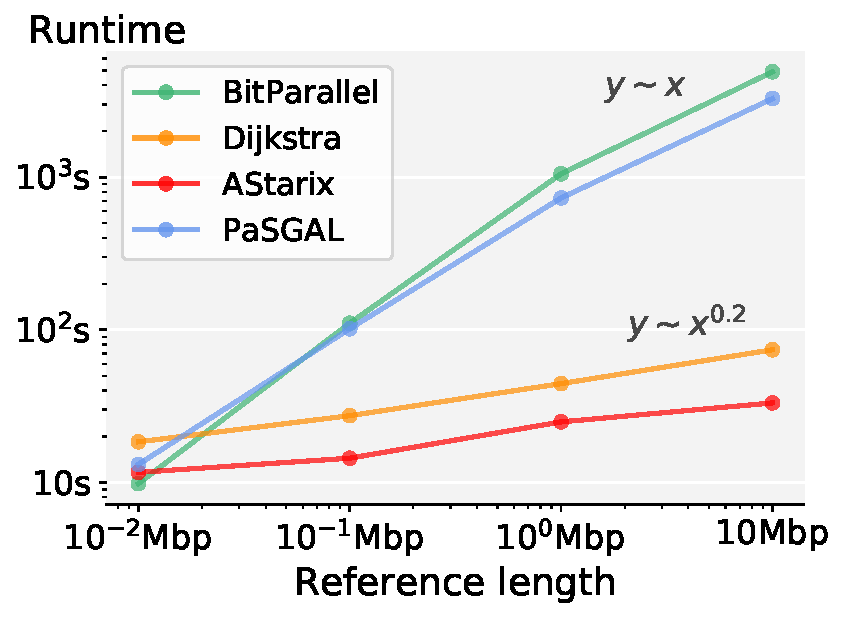
\includegraphics[width=\linewidth]{\dir/figs/cmp/performance_vs_genomesize-head_Mbpxs.pdf}
  \end{subfigure}
  \begin{subfigure}{.49\textwidth}
    \centering
    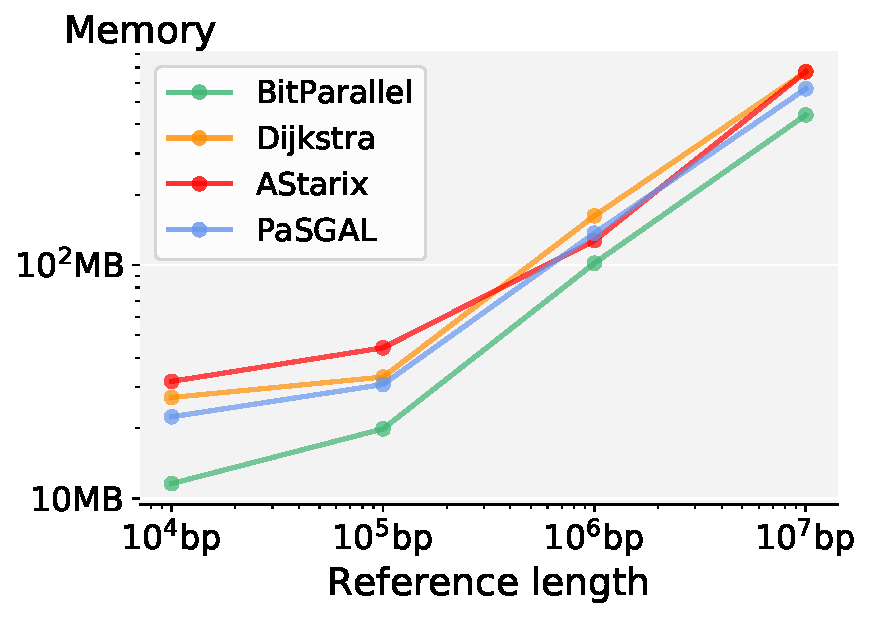
\includegraphics[width=\linewidth]{\dir/figs/cmp/memory_vs_genomesize-headxmax_rss.pdf}
  \end{subfigure}
  \caption{Comparison of overall runtime and memory usage of optimal aligners
     with increasing prefixes of E. coli as references.}
  \label{TRIEfig:scaling_with_graphsize}
\end{figure}

\subsection{\A scaling and speedup}
To measure the speedup caused by the heuristic function, we compare the number
of not only the expanded, but also of explored states (the latter number is
never smaller, see~\cref{TRIEsubsec:general-astar} and the example
in~\cref{TRIEfig:heuristic-benefit}) between \astarix and \dijkstra on the MHC1
dataset.

\cref{TRIEfig:scaling_with_errors} demonstrates the benefit of the heuristic
function in terms of both alignment time and number of explored states. Most
importantly, \astarix scales much better with increasing number of errors in the
read, compared to \dijkstra. More specifically, the number of states explored by
\dijkstra, as a function of alignment cost, grows exponentially with a base of 
around 10, whereas the base for \astarix is around 3 (the empirical complexity is
estimated as a best exponential fit \mbox{$\mli{exploredStates} \sim a \cdot
\mli{score}^b$}).

The horizontal black line in \cref{TRIEfig:scaling_with_errors} denotes the total
number of states $\lvert \RG \rvert \cdot \lvert q \rvert$, which is always
explored by \bitparallel and \pasgal. On the other hand, any aligner must
explore at least $m = \lvert q \rvert$ states, which we show as a horizontal
dashed line. This lower bound is determined by the fact that at least the states
on a best alignment need to be explored.

\begin{figure}[t]
  \begin{subfigure}{.45\textwidth}
    \centering
    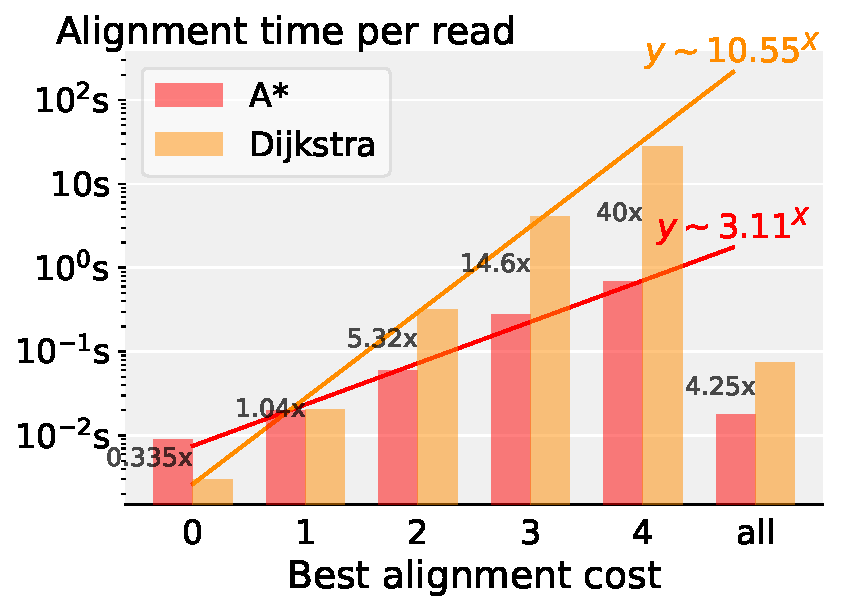
\includegraphics[width=\linewidth]{figs/cmp/heuristic_MHC1_cost-t(map).pdf}
  \end{subfigure}%~\hspace{1em}
  \begin{subfigure}{.45\textwidth}
    \centering
    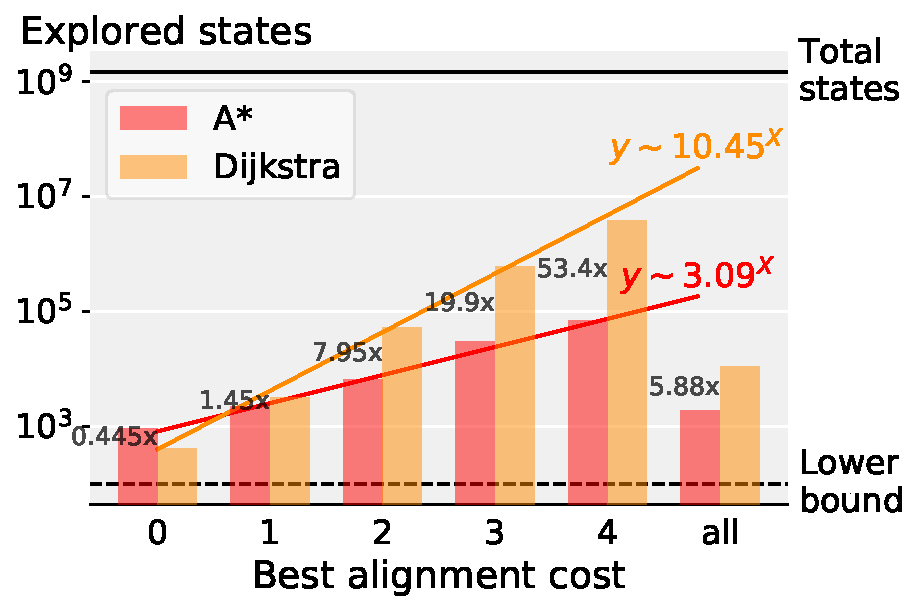
\includegraphics[width=\linewidth]{figs/cmp/heuristic_MHC1_cost-explored_states.pdf}
  \end{subfigure}%
  \caption[Performance scaling with alignment cost]{Comparison of \A and \dijkstra in terms of mean alignment runtime per read and mean explored states depending on the alignment cost on MHC1.}
  \label{TRIEfig:scaling_with_errors}
\end{figure}

